\documentclass{article}

\usepackage{fancyhdr}
\usepackage{extramarks}
\usepackage{amsmath}
\usepackage{amsthm}
\usepackage{amsfonts}
\usepackage{tikz}
\usepackage[plain]{algorithm}
\usepackage{algpseudocode}
\usepackage{xcolor}
\usepackage{amssymb}
\usepackage{todonotes}
\usepackage{mathtools}
\usepackage{cancel}
\usepackage{listings}
\usepackage{dirtytalk}
\usepackage{soul}
\usetikzlibrary{decorations.pathreplacing}
\usepackage{hyperref}
\usepackage{parcolumns}
\usepackage{tabularx}
\usepackage{caption}
\usepackage{lastpage}
\usepackage{color}
\usepackage[inline]{enumitem}


\definecolor{mygreen}{rgb}{0,0.6,0}
\definecolor{mygray}{rgb}{0.5,0.5,0.5}
\definecolor{mymauve}{rgb}{0.58,0,0.82}

\lstset{
  backgroundcolor=\color{white},   % choose the background color; you must add \usepackage{color} or \usepackage{xcolor}; should come as last argument
  basicstyle=\footnotesize,        % the size of the fonts that are used for the code
  breakatwhitespace=false,         % sets if automatic breaks should only happen at whitespace
  breaklines=true,                 % sets automatic line breaking
  captionpos=b,                    % sets the caption-position to bottom
  commentstyle=\color{mygreen},    % comment style
  deletekeywords={...},            % if you want to delete keywords from the given language
  escapeinside={\%*}{*)},          % if you want to add LaTeX within your code
  extendedchars=true,              % lets you use non-ASCII characters; for 8-bits encodings only, does not work with UTF-8
  frame=single,	                   % adds a frame around the code
  keepspaces=true,                 % keeps spaces in text, useful for keeping indentation of code (possibly needs columns=flexible)
  keywordstyle=\color{orange!90!black},       % keyword style
  language=Python,                 % the language of the code
  morekeywords={*,...},            % if you want to add more keywords to the set
  numbers=left,                    % where to put the line-numbers; possible values are (none, left, right)
  numbersep=5pt,                   % how far the line-numbers are from the code
  numberstyle=\tiny\color{mygray}, % the style that is used for the line-numbers
  rulecolor=\color{black},         % if not set, the frame-color may be changed on line-breaks within not-black text (e.g. comments (green here))
  showspaces=false,                % show spaces everywhere adding particular underscores; it overrides 'showstringspaces'
  showstringspaces=false,          % underline spaces within strings only
  showtabs=false,                  % show tabs within strings adding particular underscores
  stepnumber=1,                    % the step between two line-numbers. If it's 1, each line will be numbered
  stringstyle=\color{yellow!60!orange!80!black},     % string literal style
  tabsize=2,	                   % sets default tabsize to 2 spaces
  title=\lstname,                   % show the filename of files included with \lstinputlisting; also try caption instead of title
  keywords=[3]{self},
  keywordstyle=[3]{\color{orange!50!gray}},
  keywords=[4]{__init__, __lt__},
  keywordstyle=[4]{\color{orange!50!gray}},
  moredelim=**[is][\color{orange!90!black}]{@}{@}
}


\usetikzlibrary{automata,positioning}

%
% Basic Document Settings
%

\topmargin=-0.45in
\evensidemargin=0in
\oddsidemargin=0in
\textwidth=6.5in
\textheight=9.0in
\headsep=0.25in

\linespread{1.1}

\pagestyle{fancy}
\lhead{\hmwkAuthorName}
\chead{\hmwkClass\ (\hmwkClassInstructor): \hmwkTitle}
\rhead{\firstxmark}
\lfoot{\lastxmark}
\cfoot{Page \thepage\ of \pageref{LastPage}}

\renewcommand\headrulewidth{0.4pt}
\renewcommand\footrulewidth{0.4pt}

%
% Create Exercise Sections
%

\newcommand{\enterExerciseHeader}[1]{
    \nobreak\extramarks{}{Exercise \arabic{#1} continued on next page\ldots}\nobreak{}
    \nobreak\extramarks{Exercise \arabic{#1} (continued)}{Exercise \arabic{#1} continued on next page\ldots}\nobreak{}
}

\newcommand{\exitExerciseHeader}[1]{
    \nobreak\extramarks{Exercise \arabic{#1} (continued)}{Exercise \arabic{#1} continued on next page\ldots}\nobreak{}
    \stepcounter{#1}
    \nobreak\extramarks{Exercise \arabic{#1}}{}\nobreak{}
}

\newcount\colveccount
\newcommand*\colvec[1]{
        \global\colveccount#1
        \begin{pmatrix}
        \colvecnext
}
\def\colvecnext#1{
        #1
        \global\advance\colveccount-1
        \ifnum\colveccount>0
                \\
                \expandafter\colvecnext
        \else
                \end{pmatrix}
        \fi
}

\setcounter{secnumdepth}{0}
\newcounter{partCounter}
\newcounter{homeworkExerciseCounter}
\setcounter{homeworkExerciseCounter}{1}
\nobreak\extramarks{Exercise \arabic{homeworkExerciseCounter}}{}\nobreak{}

%
% Homework Exercise Environment
%
% This environment takes an optional argument. When given, it will adjust the
% Exercise counter. This is useful for when the Exercises given for your
% assignment aren't sequential. See the last 3 Exercises of this template for an
% example.
%
\newenvironment{homeworkExercise}[1][-1]{
    \ifnum#1>0
        \setcounter{homeworkExerciseCounter}{#1}
    \fi
    \section{Exercise \arabic{homeworkExerciseCounter}}
    \setcounter{partCounter}{1}
    \enterExerciseHeader{homeworkExerciseCounter}
}{
    \exitExerciseHeader{homeworkExerciseCounter}
}

%
% Homework Details
%   - Title
%   - Due date
%   - Class
%   - Section/Time
%   - Instructor
%   - Author
%

\newcommand{\hmwkTitle}{Assignment 5}
\newcommand{\hmwkDueDate}{May 31, 2018}
\newcommand{\hmwkClass}{Algorithms}
\newcommand{\hmwkClassTime}{Spring Semester}
\newcommand{\hmwkClassInstructor}{Prof. Antonio Carzaniga}
\newcommand{\hmwkAuthorName}{\textbf{A. Romanelli}}

%
% Title Page
%

\title{
    \vspace{2in}
    \textmd{\textbf{\hmwkClass:\ \hmwkTitle}}\\
    \normalsize\vspace{0.1in}\small{Due\ on\ \hmwkDueDate\ at 20:00}\\
    \vspace{0.1in}\large{\textit{\hmwkClassInstructor}}
    \vspace{3in}
}

\author{\hmwkAuthorName}
\date{}

\renewcommand{\part}[1]{\textbf{\large Part \Alph{partCounter}}\stepcounter{partCounter}\\}


%
% Various Helper Commands
%

% Useful for algorithms
\newcommand{\alg}[1]{\textsc{\bfseries \footnotesize #1}}

% For derivatives
\newcommand{\deriv}[1]{\frac{\mathrm{d}}{\mathrm{d}x} (#1)}

% For partial derivatives
\newcommand{\pderiv}[2]{\frac{\partial}{\partial #1} (#2)}

% Integral dx
\newcommand{\dx}{\mathrm{d}x}

% Alias for the Solution section header
\newcommand{\solution}{\textbf{\large Solution}}

% Probability commands: Expectation, Variance, Covariance, Bias
\newcommand{\E}{\mathrm{E}}
\newcommand{\Var}{\mathrm{Var}}
\newcommand{\Cov}{\mathrm{Cov}}
\newcommand{\Bias}{\mathrm{Bias}}

\begin{document}

\maketitle

\pagebreak

\begin{homeworkExercise}
	In this exercise we want to help our friend Antonio which has been studying so called \emph{irregular} subsequences. His very imaginative definition states that an irregular subsequence is such if and only if the following holds within a given sequence of integers:
	$$a_{i_1} > a_{i_2} < a_{i_3} > a_{i_4} < a_{i_5} > \dots$$
	Firstly I misinterpreted what Antonio meant, as I interpreted \emph{subsequences} as \emph{substrings} which are not really the same thing, since the possible substrings of \verb|abc| are [\verb|a|, \verb|b|, \verb|c|, \verb|ab|, \verb|bc|, \verb|abc|] whereas its subsequences are all the possible combinations also of non successive characters: [\verb|a|, \verb|b|, \verb|c|, \verb|ab|, \verb|ac|, \verb|bc|, \verb|abc|]
	\\\\ 
	Once I realised what the problem was actually asking, I felt pulled toward a Dynamic Programming approach, which would exploit recursion and the storing of partial results as I'll show you later in \textbf{Exercise 3}, but instead of going for the recursion I decided to take a easier approach in terms of both asymptotic complexity and writability.
	\subsection{Solving Strategy}
	The idea behind my solution is to linearly scan the given sequence and to compose a new sequence of operators that can be either \verb|>| or \verb|<|\ . Once this sequence is compiled, I can count how many times the operator flips and add one to count the last element considered. Let's take a look at some more concrete examples:
	$$\text{The sequence: } [0,\ 4,\ 2,\ 3,\ 3]\ \text{has the following relationships:}$$
	$$0 < \color{red}4 > 2 < 3 \color{black}= 3,\ \text{thus our operators' sequence will be:}$$
	$$[>, <] \implies 3$$\\
	We can now just count the elements in our operators' sequence and add one to find what's the longest possible subsequence that satisfies such a property like the \emph{irregular} one.\\\\
	\begin{minipage}{0.33\textwidth}
		$$[1,\ 2,\ 3,\ 4]$$
		$$1 < 2 < 3 < 4$$
		$$[<] \implies 2$$
	\end{minipage}
	\begin{minipage}{0.33\textwidth}
		$$[2,\ 1,\ 2,\ 1,\ 2]$$
		$$2 > 1 < 2 > 1 < 2$$
		$$[>, <, >, <] \implies 5$$
	\end{minipage}
	\begin{minipage}{0.33\textwidth}
		$$[0,\ 4,\ 3,\ 0,\ 0,\ 2,\ 2,\ 3,\ 4]$$
		$$0 < 4 > 3 > 0 = 0 < 2 = 2 < 3 < 4$$
		$$[>, <] \implies 3$$
	\end{minipage}\\\\\\
	Now that the strategy is clear, I should better explain how I can get from a given sequence to the correct operators' sequence.
	\subsection{Implementation}
	This time around I don't have to go about how my data structure works so I'll try to be as brief as possible, the code you're about to see is the product of condensing and refactoring to minimal terms the code to avoid redundancies.
	\begin{lstlisting}
A = []
for n in input().split():
	A.append(int(n))\end{lstlisting}
\vspace{-0.75cm}
As always we need to parse the input from a string into sensible data.
\newpage
Once we are done with the parsing we can get to work:
\begin{lstlisting}[firstnumber=4]
def lenOfIrregEx(A):
	if len(A) < 2:
	    return len(A)
	signs = []
	for i in range(1,len(A)):
	    if A[i-1] > A[i]:
	        if len(signs) == 0 or signs[-1] != ">":
	            signs.append(">")
	    elif A[i-1] < A[i]:
	        if len(signs) != 0 and signs[-1] != "<":
	            signs.append("<")
	return len(signs) + 1\end{lstlisting}
\vspace{-0.75cm}
In the first two lines of this function I handle the case whether our array consists of less than two elements, in which cases we really can't compare anything but we know already the solutions to such problems. \\ \\
Else the first thing to do is \textemdash\ after allocating the \verb|signs| array \textemdash\ to linearly scan the given sequence.
I do \underline{not} want to append to the \verb|signs| array \underline{every} operator that I'm able to find, but only those that make sense to count, thus if I have \verb|>| and \verb|>| as its successive, it would not make sense to append the second one. What I'm interested in is to append an operator only when it's different from the last one I have appended. Moreover I do not want my operator list to start with a \verb|<| but exclusively with \verb|>|\ . \\ \\
The conditions on which I decide to append (or not) an operator to my array should now be clearer.
The very last thing we are left to do is to simply count how many operators I have at the end of the scan and add 1.

\subsection{Time Complexity Analysis}
As I previously described, the only thing we are doing is a linear scan of the array and for each element we'll append it to our operators' array if that's the case. Our best case scenario is that we don't have anything to append and thus we only take $n$ time. \\ \\Our worst case happens when the whole sequence is an irregular one. But what does this imply? \\ \\
	If our whole sequence is irregular, then we will need to allocate $n-1$ operators within the operators array and \textemdash\ as we all know \textemdash\ appending an element to an array takes $\mathcal{O}(c)$ and since we would do it for $n-1$ elements this gives us a worst case complexity of: $c(n-1)$. \\ \\
	Thus we can conclude that this code runs in $\mathcal{O}(n)$
\end{homeworkExercise}
\newpage
\begin{homeworkExercise}
	This time around, our pal Antonio has given us a $n \times m$ grid, just like the one we had created in \textbf{Assignment 4}, where we were looking for the shortest path out of a maze. According to his ever so imaginative vocabulary, he decided to denote a specific sequence of adjacent cells of this grid as \emph{interesting} path if every value in a cell is greater than its preceding one. Our goal is to return the length of the longest \emph{interesting} path.
\subsection{Assets}
As in the previous assignment, I recycled the structures of a \verb|Cell| and \verb|Grid|. The latter stayed the same where I slightly modified the \verb|Cell| structure to fit my needs:
\lstinputlisting[firstline=1, lastline=21, firstnumber=1, title=Data Structure for the \texttt{Grid} and \texttt{Cell}]{ex2bis.py}
I also recycled the input parser, which is going to allocate the grid depending on the first two integers passed from the standard input and then allocate one row at a time:
\lstinputlisting[firstline=55, lastline=65, firstnumber=1, title=Input parser for a $n \times m$ \texttt{Grid} allocation]{ex2bis.py}
\subsection{Solving Strategy}
The intuition that was most helpful in solving this problem came to me when I took a look at the proposed complexity of $\mathcal{O}(nm \log(nm))$, this pointed me towards the fact that I could exploit a sorting algorithm and the fact that the \emph{interesting} path must account for a number being greater than its predecessor. \\
The idea behind my solution is to allocate a linear array of cells and to sort them in ascending order using the built-in function provided by \textbf{Python}, then setting the base case to be the first element of this newly created array, which will have a longest length of 0: the \emph{interesting} path that terminates in the considered cell. \\\\
Then from left to right I'm going to compute the length of the longest path exploiting the base case that we just set and checking whether there are adjacent cells that have lesser key than the one we are considering.
\begin{figure}[h]
\centering
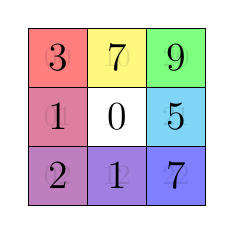
\begin{tikzpicture}[scale=0.75]
	\fill[color=red, opacity=0.5] (0,0) rectangle (1,1);
	\fill[color=yellow, opacity=0.5] (1,0) rectangle (2,1);
	\fill[color=green, opacity=0.5] (2,0) rectangle (3,1);
	\fill[color=red!50!violet, opacity=0.5] (0,-1) rectangle (1,0);
	\fill[color=white] (1,-1) rectangle (2,0);
	\fill[color=cyan, opacity=0.5] (2,-1) rectangle (3,0); 
	\fill[color=violet, opacity=0.5] (0,-2) rectangle (1,-1);
	\fill[color=violet!50!blue, opacity=0.5] (1,-2) rectangle (2,-1);
	\fill[color=blue, opacity=0.5] (2,-2) rectangle (3,-1);
	\foreach \x in {0,...,2} {
		\foreach \y in {0,...,2} {
			\draw (\x,-\y) rectangle (\x+1, -\y+1);
			\node[opacity=0.1] at (\x+0.5, -\y+0.5) {\x\y};
		}
	}
	\node at (0.5, 0.5) {\Large 3};
	\node at (0.5, -0.5) {\Large 1};
	\node at (0.5, -1.5) {\Large 2};
	\node at (1.5, 0.5) {\Large 7};
	\node at (1.5, -0.5) {\Large 0};
	\node at (1.5, -1.5) {\Large 1};
	\node at (2.5, 0.5) {\Large 9};
	\node at (2.5, -0.5) {\Large 5};
	\node at (2.5, -1.5) {\Large 7};
\end{tikzpicture}\\
\vspace{1cm}
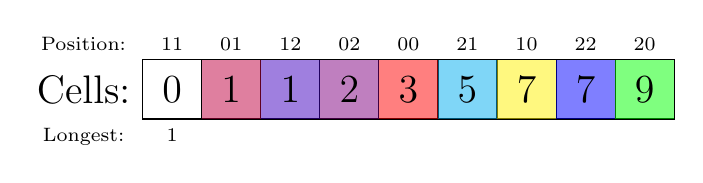
\begin{tikzpicture}[scale=0.75]
	\foreach \x in {0, ..., 8} {
		\draw (\x, 0) rectangle (\x+1, 1);
	}
	\node at (0.5, 0.5) {\Large 0};
	\node[anchor=south] at (0.5, 1) {\scriptsize 11};
	\fill[color=red!50!violet, opacity=0.5] (1,0) rectangle (2,1);
	\node[anchor=south] at (1.5, 1) {\scriptsize 01};
	\node at (1.5, 0.5) {\Large 1};
	\fill[color=violet!50!blue, opacity=0.5] (2,0) rectangle (3,1);
	\node[anchor=south] at (2.5, 1) {\scriptsize 12};
	\node at (2.5, 0.5) {\Large 1};
	\fill[color=violet, opacity=0.5] (3,0) rectangle (4,1);
	\node[anchor=south] at (3.5, 1) {\scriptsize 02};
	\node at (3.5, 0.5) {\Large 2};
	\fill[color=red, opacity=0.5] (4,0) rectangle (5,1);
	\node[anchor=south] at (4.5, 1) {\scriptsize 00};
	\node at (4.5, 0.5) {\Large 3};
	\fill[color=cyan, opacity=0.5] (5,0) rectangle (6,1);
	\node[anchor=south] at (5.5, 1) {\scriptsize 21};
	\node at (5.5, 0.5) {\Large 5};
	\fill[color=yellow, opacity=0.5] (6,0) rectangle (7,1);
	\node[anchor=south] at (6.5, 1) {\scriptsize 10};
	\node at (6.5, 0.5) {\Large 7};
	\fill[color=blue, opacity=0.5] (7,0) rectangle (8,1);
	\node[anchor=south] at (7.5, 1) {\scriptsize 22};
	\node at (7.5, 0.5) {\Large 7};
	\fill[color=green, opacity=0.5] (8,0) rectangle (9,1);
	\node[anchor=south] at (8.5, 1) {\scriptsize 20};
	\node at (8.5, 0.5) {\Large 9};
	
	\node[anchor=north] at (0.5, 0) {\scriptsize 1};
	
	\node[anchor=north] at (-1, 0) {\scriptsize Longest:};
	
	\node[anchor=south] at (-1, 1) {\scriptsize Position:};
	\node at (-1, 0.5) {\Large Cells:};
\end{tikzpicture}
\end{figure} \\
Now that we have our linear array and our base case that the cell 0 at position 11, besides having four adjacent cells, since it's the minimum of the array, it cannot be the ending cell of a sequence longer than 1. \\ \\
If we want to compute the longest sequence for a given cell, it's enough to consider its adjacent cells that have a key lesser than the considered one \textemdash\ thus implying that we already computed the adjacent cell longest path \textemdash\ and simply add one to the maximum longest path of the adjacent cells that we managed to find. \\ \\
\begin{minipage}{0.5\linewidth}
	\centering
	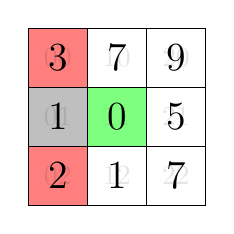
\begin{tikzpicture}[scale=0.75]
		\fill[color=red, opacity=0.5] (0,0) rectangle (1,1);
%		\fill[color=yellow, opacity=0.5] (1,0) rectangle (2,1);
%		\fill[color=green, opacity=0.5] (2,0) rectangle (3,1);
		\fill[color=black, opacity=0.25] (0,-1) rectangle (1,0);
		\fill[color=green, opacity=0.5] (1,-1) rectangle (2,0);
%		\fill[color=cyan, opacity=0.5] (2,-1) rectangle (3,0); 
		\fill[color=red, opacity=0.5] (0,-2) rectangle (1,-1);
%		\fill[color=violet!50!blue, opacity=0.5] (1,-2) rectangle (2,-1);
%		\fill[color=blue, opacity=0.5] (2,-2) rectangle (3,-1);
		\foreach \x in {0,...,2} {
			\foreach \y in {0,...,2} {
				\draw (\x,-\y) rectangle (\x+1, -\y+1);
				\node[opacity=0.1] at (\x+0.5, -\y+0.5) {\x\y};
			}
		}
		\node at (0.5, 0.5) {\Large 3};
		\node at (0.5, -0.5) {\Large 1};
		\node at (0.5, -1.5) {\Large 2};
		\node at (1.5, 0.5) {\Large 7};
		\node at (1.5, -0.5) {\Large 0};
		\node at (1.5, -1.5) {\Large 1};
		\node at (2.5, 0.5) {\Large 9};
		\node at (2.5, -0.5) {\Large 5};
		\node at (2.5, -1.5) {\Large 7};
	\end{tikzpicture}\\
	\vspace{1cm}
	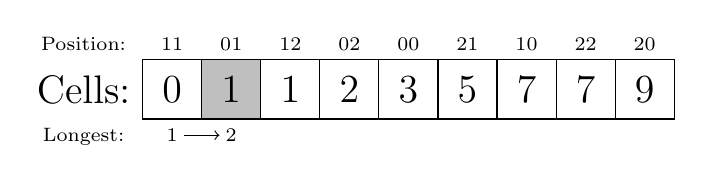
\begin{tikzpicture}[scale=0.75]
		\foreach \x in {0, ..., 8} {
			\draw (\x, 0) rectangle (\x+1, 1);
		}
		\node at (0.5, 0.5) {\Large 0};
		\node[anchor=south] at (0.5, 1) {\scriptsize 11};
		\fill[color=black, opacity=0.25] (1,0) rectangle (2,1);
		\node[anchor=south] at (1.5, 1) {\scriptsize 01};
		\node at (1.5, 0.5) {\Large 1};
%		\fill[color=violet!50!blue, opacity=0.5] (2,0) rectangle (3,1);
		\node[anchor=south] at (2.5, 1) {\scriptsize 12};
		\node at (2.5, 0.5) {\Large 1};
%		\fill[color=violet, opacity=0.5] (3,0) rectangle (4,1);
		\node[anchor=south] at (3.5, 1) {\scriptsize 02};
		\node at (3.5, 0.5) {\Large 2};
%		\fill[color=red, opacity=0.5] (4,0) rectangle (5,1);
		\node[anchor=south] at (4.5, 1) {\scriptsize 00};
		\node at (4.5, 0.5) {\Large 3};
%		\fill[color=cyan, opacity=0.5] (5,0) rectangle (6,1);
		\node[anchor=south] at (5.5, 1) {\scriptsize 21};
		\node at (5.5, 0.5) {\Large 5};
%		\fill[color=yellow, opacity=0.5] (6,0) rectangle (7,1);
		\node[anchor=south] at (6.5, 1) {\scriptsize 10};
		\node at (6.5, 0.5) {\Large 7};
%		\fill[color=blue, opacity=0.5] (7,0) rectangle (8,1);
		\node[anchor=south] at (7.5, 1) {\scriptsize 22};
		\node at (7.5, 0.5) {\Large 7};
%		\fill[color=green, opacity=0.5] (8,0) rectangle (9,1);
		\node[anchor=south] at (8.5, 1) {\scriptsize 20};
		\node at (8.5, 0.5) {\Large 9};
		
		\node[anchor=north] at (0.5, 0) {\scriptsize 1};
		\draw[->] (0.7, -0.275) -- (1.3, -0.275);
		\node[anchor=north] at (1.5, 0) {\scriptsize 2};
		
		\node[anchor=north] at (-1, 0) {\scriptsize Longest:};
		
		\node[anchor=south] at (-1, 1) {\scriptsize Position:};
		\node at (-1, 0.5) {\Large Cells:};
	\end{tikzpicture}
\end{minipage}
\begin{minipage}{0.5\linewidth}
	\centering
	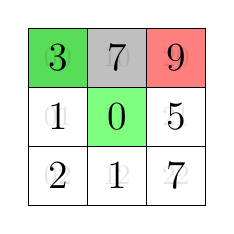
\begin{tikzpicture}[scale=0.75]
		\fill[color=green!80!black, opacity=0.66] (0,0) rectangle (1,1);
		\fill[color=black, opacity=0.25] (1,0) rectangle (2,1);
		\fill[color=red, opacity=0.5] (2,0) rectangle (3,1);
%		\fill[color=black, opacity=0.25] (0,-1) rectangle (1,0);
		\fill[color=green, opacity=0.5] (1,-1) rectangle (2,0);
%		\fill[color=cyan, opacity=0.5] (2,-1) rectangle (3,0); 
%		\fill[color=red, opacity=0.5] (0,-2) rectangle (1,-1);
%		\fill[color=violet!50!blue, opacity=0.5] (1,-2) rectangle (2,-1);
%		\fill[color=blue, opacity=0.5] (2,-2) rectangle (3,-1);
		\foreach \x in {0,...,2} {
			\foreach \y in {0,...,2} {
				\draw (\x,-\y) rectangle (\x+1, -\y+1);
				\node[opacity=0.1] at (\x+0.5, -\y+0.5) {\x\y};
			}
		}
		\node at (0.5, 0.5) {\Large 3};
		\node at (0.5, -0.5) {\Large 1};
		\node at (0.5, -1.5) {\Large 2};
		\node at (1.5, 0.5) {\Large 7};
		\node at (1.5, -0.5) {\Large 0};
		\node at (1.5, -1.5) {\Large 1};
		\node at (2.5, 0.5) {\Large 9};
		\node at (2.5, -0.5) {\Large 5};
		\node at (2.5, -1.5) {\Large 7};
	\end{tikzpicture}\\
	\vspace{1cm}
	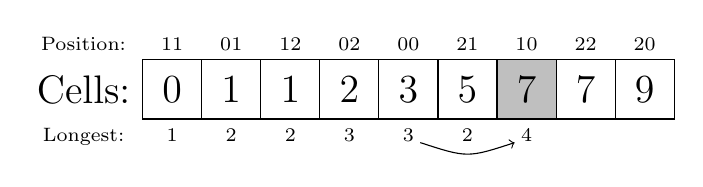
\begin{tikzpicture}[scale=0.75]
		\foreach \x in {0, ..., 8} {
			\draw (\x, 0) rectangle (\x+1, 1);
		}
		\node at (0.5, 0.5) {\Large 0};
		\node[anchor=south] at (0.5, 1) {\scriptsize 11};
		\node[anchor=south] at (1.5, 1) {\scriptsize 01};
		\node at (1.5, 0.5) {\Large 1};
%		\fill[color=violet!50!blue, opacity=0.5] (2,0) rectangle (3,1);
		\node[anchor=south] at (2.5, 1) {\scriptsize 12};
		\node at (2.5, 0.5) {\Large 1};
%		\fill[color=violet, opacity=0.5] (3,0) rectangle (4,1);
		\node[anchor=south] at (3.5, 1) {\scriptsize 02};
		\node at (3.5, 0.5) {\Large 2};
%		\fill[color=red, opacity=0.5] (4,0) rectangle (5,1);
		\node[anchor=south] at (4.5, 1) {\scriptsize 00};
		\node at (4.5, 0.5) {\Large 3};
%		\fill[color=cyan, opacity=0.5] (5,0) rectangle (6,1);
		\node[anchor=south] at (5.5, 1) {\scriptsize 21};
		\node at (5.5, 0.5) {\Large 5};
%		\fill[color=yellow, opacity=0.5] (6,0) rectangle (7,1);
		\node[anchor=south] at (6.5, 1) {\scriptsize 10};
		\node at (6.5, 0.5) {\Large 7};
%		\fill[color=blue, opacity=0.5] (7,0) rectangle (8,1);
		\node[anchor=south] at (7.5, 1) {\scriptsize 22};
		\fill[color=black, opacity=0.25] (6,0) rectangle (7,1);
		\node at (7.5, 0.5) {\Large 7};
%		\fill[color=green, opacity=0.5] (8,0) rectangle (9,1);
		\node[anchor=south] at (8.5, 1) {\scriptsize 20};
		\node at (8.5, 0.5) {\Large 9};
		
		\node[anchor=north] at (0.5, 0) {\scriptsize 1};
		\node[anchor=north] at (1.5, 0) {\scriptsize 2};
		\node[anchor=north] at (2.5, 0) {\scriptsize 2};
		\node[anchor=north] at (3.5, 0) {\scriptsize 3};
		\node[anchor=north] at (4.5, 0) {\scriptsize 3};
		\node[anchor=north] at (5.5, 0) {\scriptsize 2};
		\draw[->] (4.7, -0.4) .. controls (5.5,-0.66) .. (6.3, -0.4);
		\node[anchor=north] at (6.5, 0) {\scriptsize 4};
		
		\node[anchor=north] at (-1, 0) {\scriptsize Longest:};
		
		\node[anchor=south] at (-1, 1) {\scriptsize Position:};
		\node at (-1, 0.5) {\Large Cells:};
	\end{tikzpicture}
\end{minipage} \\ \\ \\
As we keep computing the longest distance for every cell, it's going to be easy to keep track of the longest one we found so far and to return at the end of our process, solving the problem.
\subsection{Implementation}
My implementation is quite straight forward and should not require any further explanation as it follows 1:1 my solving strategy:
\begin{itemize}
	\item Generate array sorted array of cells;
	\item Compute distance by watching adjacent cells that were already computed;
	\item Return the longest distance ever computed.
\end{itemize}
\lstinputlisting[firstline=22, lastline=54, firstnumber=24, title=Implementation of the solving strategy]{ex2bis.py}
\subsection{Time Complexity Analysis}
In this exercise sorting the array came at a cost of complexity, which as we know is $\mathcal{O}(n \log n)$, but since we sorted an array of cells of our $n \times m$ grid, we effectively sorted $nm$ cells, thus our asymptotic complexity so far is going to be: $\mathcal{O}(nm \log (nm))$.
The rest of our implementation can be trivially seen to be linear over the number of cells, which does not affect our complexity. This means that our complexity is going to match the requirements for this assignment:
$$\mathcal{O}(nm \log (nm))$$
\end{homeworkExercise}
\newpage
\begin{homeworkExercise}
	Antonio's obsession this exercise is about palindromic subsequences and more specifically he wants to know, given a string, what's the longest palindromic subsequence present in the string. Just like in the first exercise, there was a possible misunderstanding of the difference between substring and subsequence. Specifically:
	\begin{center}
		abracadabra
	\end{center}
	Has a palindromic subsequence of length 7, you don't believe me?
	\begin{center}
		\color{red}ab\color{black}rac\color{red}adab\color{black}r\color{red}a\color{black}\\
		\color{red}abadaba\color{black}\\
		\vspace{-0.25cm}
		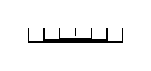
\begin{tikzpicture}
			\draw (0,0) -- (0,0.1);
			\draw (-0.2,0.1) -- (-0.2, -0.025) -- (0.2,-0.025) -- (0.2, 0.1);
			\draw (-0.4,0.1) -- (-0.4, -0.05) -- (0.4,-0.05) -- (0.4, 0.1);
			\draw (-0.6,0.1) -- (-0.6, -0.075) -- (0.6,-0.075) -- (0.6, 0.1);
		\end{tikzpicture}
	\end{center}
	\subsection{Solving Strategy}
	The initial idea would be to solve this problem by means of recursion, checking all the possible subsequences that there are but we would soon run out of time complexity, as the numbers of subsequences to check grows exponentially. \\ \\
	The concept of dynamic programming that we recently studied in class could turn out useful. We know that our base case will be for the subsequence of length 1, which must also have length 1. If we then have a tree which has at its root our string and as its children all the possible subsequences:
	\begin{figure}[h]
		\centering
		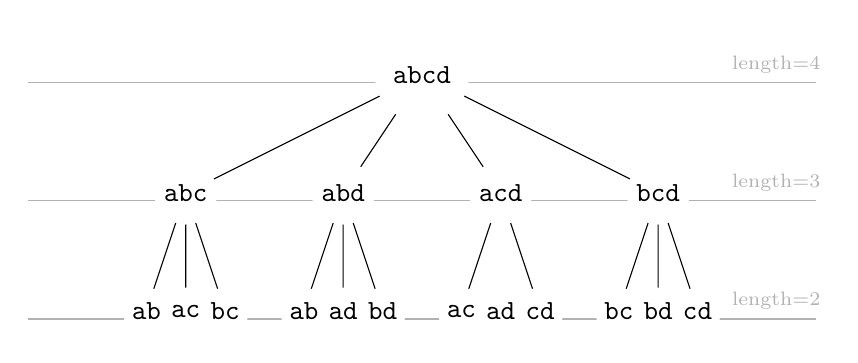
\begin{tikzpicture}
			\draw[opacity=0.3] (-5,-0.1) -- (5,-0.1)
				node[above,pos=0.95] {\scriptsize length=4};
			\draw[opacity=0.3] (-5,-1.6) -- (5,-1.6)
				node[above,pos=0.95] {\scriptsize length=3};
			\draw[opacity=0.3] (-5,-3.1) -- (5,-3.1)
				node[above,pos=0.95] {\scriptsize length=2};
			
			
			\draw (3,-1.5) -- (0,0) -- (1,-1.5) -- (0,0) -- (-1,-1.5) -- (0,0) -- (-3,-1.5);
			\draw (-3.5,-3) -- (-3,-1.5) -- (-2.5,-3) -- (-3,-1.5) -- (-3,-3);
			\draw (-1.5,-3) -- (-1,-1.5) -- (-0.5,-3)  -- (-1,-1.5)  -- (-1,-3);
			\draw (3.5,-3) -- (3,-1.5) -- (2.5,-3) -- (3,-1.5) -- (3,-3);
			\draw (1.5,-3) -- (1,-1.5) -- (0.5,-3);			
			\fill[white] (0,0) circle (0.6cm);
			\fill[white] (-3,-1.5) circle (0.4cm);
			\fill[white] (-1,-1.5) circle (0.4cm);
			\fill[white] (1,-1.5) circle (0.4cm);
			\fill[white] (3,-1.5) circle (0.4cm);
			\fill[white] (-3.5,-3) circle (0.3cm);
			\fill[white] (-3,-3) circle (0.3cm);
			\fill[white] (-2.5,-3) circle (0.3cm);
			\fill[white] (-1.5,-3) circle (0.3cm);
			\fill[white] (-1,-3) circle (0.3cm);
			\fill[white] (-0.5,-3) circle (0.3cm);
			\fill[white] (0.5,-3) circle (0.3cm);
			\fill[white] (1,-3) circle (0.3cm);
			\fill[white] (1.5,-3) circle (0.3cm);
			\fill[white] (2.5,-3) circle (0.3cm);
			\fill[white] (3,-3) circle (0.3cm);
			\fill[white] (3.5,-3) circle (0.3cm);
			
			
			\node at (0,0) {\verb|abcd|};
			
			\node at (-3,-1.5) {\verb|abc|};
			\node at (-1,-1.5) {\verb|abd|};
			\node at (1, -1.5) {\verb|acd|};
			\node at (3, -1.5) {\verb|bcd|};
			
			\node at (-3.5,-3) {\verb|ab|};
			\node at (-3,-3) {\verb|ac|};
			\node at (-2.5,-3) {\verb|bc|};
			\node at (-1,-3) {\verb|ad|};
			\node at (-1.5,-3) {\verb|ab|};
			\node at (-0.5,-3) {\verb|bd|};
			\node at (0.5, -3) {\verb|ac|};
			\node at (1, -3) {\verb|ad|};
			\node at (1.5, -3) {\verb|cd|};
			\node at (2.5, -3) {\verb|bc|};	
			\node at (3, -3) {\verb|bd|};	
			\node at (3.5, -3) {\verb|cd|};		
			
			
		\end{tikzpicture}
		\caption{All possible subsequences for \texttt{abcd}}
	\end{figure} \\
	Something worth noticing is how we considered multiple times the same subsequences which means that we are going to spend time trying to compute something we already did previously, which hint the fact that we should store partial subproblem solutions using the tabulation method. \\ \\
	If we consider an actual palindrome subsequence like:
	\begin{figure}[H]
		\centering
		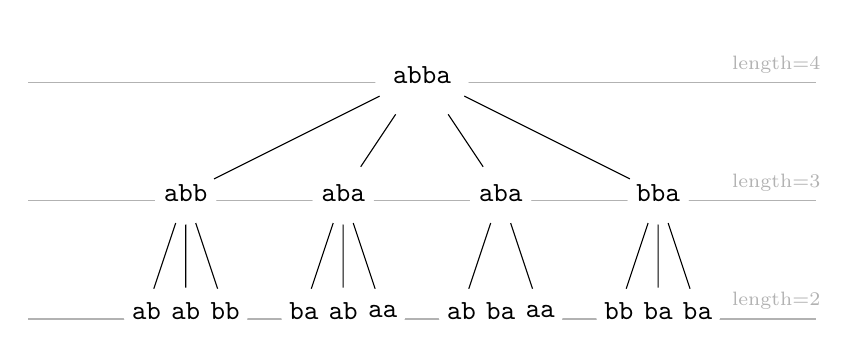
\begin{tikzpicture}
			\draw[opacity=0.3] (-5,-0.1) -- (5,-0.1)
				node[above,pos=0.95] {\scriptsize length=4};
			\draw[opacity=0.3] (-5,-1.6) -- (5,-1.6)
				node[above,pos=0.95] {\scriptsize length=3};
			\draw[opacity=0.3] (-5,-3.1) -- (5,-3.1)
				node[above,pos=0.95] {\scriptsize length=2};
			
			
			\draw (3,-1.5) -- (0,0) -- (1,-1.5) -- (0,0) -- (-1,-1.5) -- (0,0) -- (-3,-1.5);
			\draw (-3.5,-3) -- (-3,-1.5) -- (-2.5,-3) -- (-3,-1.5) -- (-3,-3);
			\draw (-1.5,-3) -- (-1,-1.5) -- (-0.5,-3)  -- (-1,-1.5)  -- (-1,-3);
			\draw (3.5,-3) -- (3,-1.5) -- (2.5,-3) -- (3,-1.5) -- (3,-3);
			\draw (1.5,-3) -- (1,-1.5) -- (0.5,-3);			
			\fill[white] (0,0) circle (0.6cm);
			\fill[white] (-3,-1.5) circle (0.4cm);
			\fill[white] (-1,-1.5) circle (0.4cm);
			\fill[white] (1,-1.5) circle (0.4cm);
			\fill[white] (3,-1.5) circle (0.4cm);
			\fill[white] (-3.5,-3) circle (0.3cm);
			\fill[white] (-3,-3) circle (0.3cm);
			\fill[white] (-2.5,-3) circle (0.3cm);
			\fill[white] (-1.5,-3) circle (0.3cm);
			\fill[white] (-1,-3) circle (0.3cm);
			\fill[white] (-0.5,-3) circle (0.3cm);
			\fill[white] (0.5,-3) circle (0.3cm);
			\fill[white] (1,-3) circle (0.3cm);
			\fill[white] (1.5,-3) circle (0.3cm);
			\fill[white] (2.5,-3) circle (0.3cm);
			\fill[white] (3,-3) circle (0.3cm);
			\fill[white] (3.5,-3) circle (0.3cm);
			
			
			\node at (0,0) {\verb|abba|};
			
			\node at (-3,-1.5) {\verb|abb|};
			\node at (-1,-1.5) {\verb|aba|};
			\node at (1, -1.5) {\verb|aba|};
			\node at (3, -1.5) {\verb|bba|};
			
			\node at (-3.5,-3) {\verb|ab|};
			\node at (-3,-3) {\verb|ab|};
			\node at (-2.5,-3) {\verb|bb|};
			\node at (-1,-3) {\verb|ab|};
			\node at (-1.5,-3) {\verb|ba|};
			\node at (-0.5,-3) {\verb|aa|};
			\node at (0.5, -3) {\verb|ab|};
			\node at (1, -3) {\verb|ba|};
			\node at (1.5, -3) {\verb|aa|};
			\node at (2.5, -3) {\verb|bb|};	
			\node at (3, -3) {\verb|ba|};	
			\node at (3.5, -3) {\verb|ba|};		
		\end{tikzpicture}
		\caption{All possible subsequences for \texttt{abba}}
	\end{figure}
	\noindent We can find out the length of the longest palindromic subsequence by starting from our leaves and doing solving the subproblems bottom-upwards.\\\\
	If the first and last characters of a subsequence of length n match, then we take the value stored in the sub-subsequence of length n-2 and add 2 to it, whereas if they don't match we just carry on the bottom highest value from the children of the node. We should also consider the case where if we are considering subsequences of length 2 and we find a match, since we cannot look for a subsequence of length 2-2 = 0, we need to explicitly set the new highest value to be 2. \\ \\
	Starting from the individual characters \textemdash\ thus the length of the longest palindromic subsequence is 1 \textemdash\ the program will build a tree bottoms up, starting from the base cases:
	\begin{figure}[h]
		\centering
		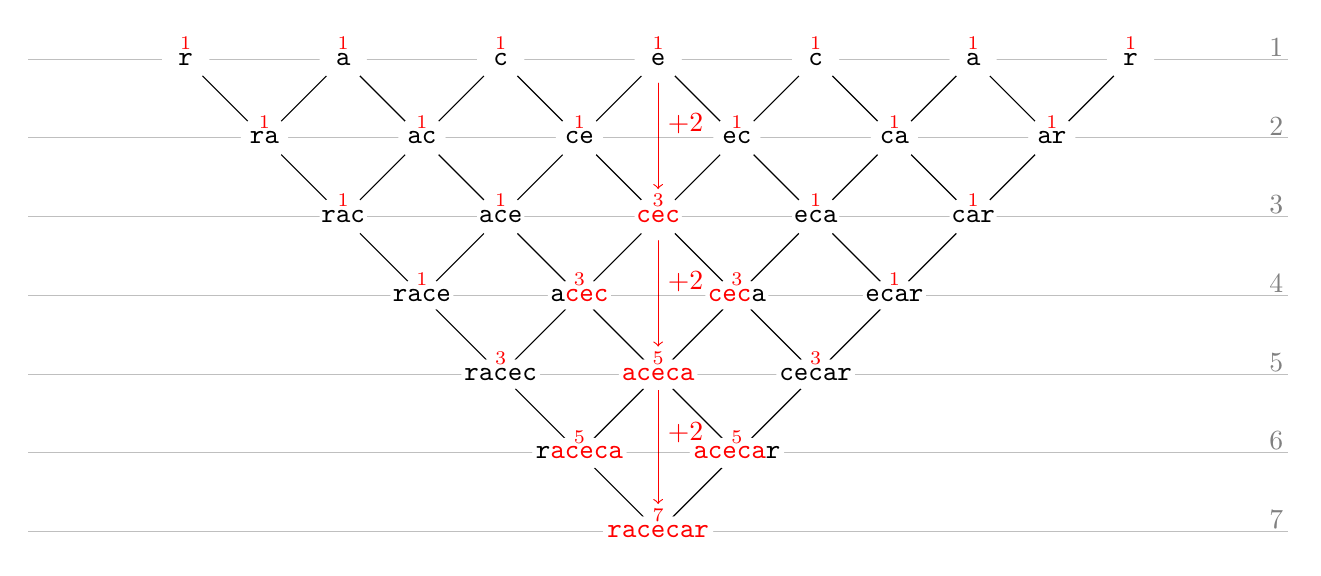
\begin{tikzpicture}
		
			\draw (-6,0) -- (0,-6) -- (6,0);
			
			\draw (-4,0) -- (1,-5);
			\draw (-2,0) -- (2,-4);
			\draw (0,0) --  (3,-3);
			\draw (2,0) -- (4,-2);
			\draw (4,0) -- (5,-1);
			
			\draw (4,0) -- (-1,-5);
			\draw (2,0) -- (-2,-4);
			\draw (0,0) -- (-3,-3);
			\draw (-2,0) -- (-4,-2);
			\draw (-4,0) -- (-5,-1);
			
			\draw[->, red] (0,0) -- (0, -1.65)
				node[right,pos=0.5] {+2};
				
			\draw[->, red] (0,-2) -- (0, -3.65)
				node[right,pos=0.5] {+2};
				
			\draw[->, red] (0,-4) -- (0, -5.65)
				node[right,pos=0.45] {+2};
										
			\draw[opacity=0.25] (-8, 0) -- (8,0);
			\fill[fill=white] (-6,0) circle (0.3cm)
				node {\texttt{r}}
				node[anchor=south] {\scriptsize \color{red} 1};
			\fill[fill=white] (-4,0) circle (0.3cm)
				node {\texttt{a}}		
				node[anchor=south] {\scriptsize \color{red} 1};
			\fill[fill=white] (-2,0) circle (0.3cm)
				node {\texttt{c}}
				node[anchor=south] {\scriptsize \color{red} 1};			
			\fill[fill=white] (0,0) circle (0.3cm)
				node {\texttt{e}}
				node[anchor=south] {\scriptsize \color{red} 1};
			\fill[fill=white] (2,0) circle (0.3cm)
				node {\texttt{c}}
				node[anchor=south] {\scriptsize \color{red} 1};
			\fill[fill=white] (4,0) circle (0.3cm)
				node {\texttt{a}}
				node[anchor=south] {\scriptsize \color{red} 1};
			\fill[fill=white] (6,0) circle (0.3cm)
				node {\texttt{r}}
				node[anchor=south] {\scriptsize \color{red} 1};
				
			\draw[opacity=0.25] (-8, -1) -- (8,-1);
			\fill[fill=white] (-5,-1) circle (0.3cm)
				node {\texttt{ra}}
				node[anchor=south] {\scriptsize \color{red} 1};
			\fill[fill=white] (-3,-1) circle (0.3cm)
				node {\texttt{ac}}
				node[anchor=south] {\scriptsize \color{red} 1};
			\fill[fill=white] (-1,-1) circle (0.3cm)
				node {\texttt{ce}}
				node[anchor=south] {\scriptsize \color{red} 1};
			\fill[fill=white] (1,-1) circle (0.3cm)
				node {\texttt{ec}}
				node[anchor=south] {\scriptsize \color{red} 1};
			\fill[fill=white] (3,-1) circle (0.3cm)
				node {\texttt{ca}}
				node[anchor=south] {\scriptsize \color{red} 1};
			\fill[fill=white] (5,-1) circle (0.3cm)
				node {\texttt{ar}}
				node[anchor=south] {\scriptsize \color{red} 1};
				
			\draw[opacity=0.25] (-8, -2) -- (8,-2);
			\fill[fill=white] (-4,-2) circle (0.3cm)
				node {\texttt{rac}}
				node[anchor=south] {\scriptsize \color{red} 1};
			\fill[fill=white] (-2,-2) circle (0.3cm)
				node {\texttt{ace}}
				node[anchor=south] {\scriptsize \color{red} 1};
			\fill[fill=white] (0,-2) circle (0.3cm)
				node {\texttt{\color{red}cec}}
				node[anchor=south] {\scriptsize \color{red} 3};		
			\fill[fill=white] (2,-2) circle (0.3cm)
				node {\texttt{eca}}
				node[anchor=south] {\scriptsize \color{red} 1};
			\fill[fill=white] (4,-2) circle (0.3cm)
				node {\texttt{car}}
				node[anchor=south] {\scriptsize \color{red} 1};
				
			\draw[opacity=0.25] (-8, -3) -- (8,-3);
			\fill[fill=white] (-3,-3) ellipse (0.4cm and 0.2cm)
				node {\texttt{race}}
				node[anchor=south] {\scriptsize \color{red} 1};
			\fill[fill=white] (-1,-3) ellipse (0.4cm and 0.2cm)
				node {\texttt{a\color{red}cec}}
				node[anchor=south] {\scriptsize \color{red} 3};
			\fill[fill=white] (1,-3) ellipse (0.4cm and 0.2cm)
				node {\texttt{\color{red}cec\color{black}a}}
				node[anchor=south] {\scriptsize \color{red} 3};
			\fill[fill=white] (3,-3) ellipse (0.4cm and 0.2cm)
				node {\texttt{ecar}}
				node[anchor=south] {\scriptsize \color{red} 1};
							
			\draw[opacity=0.25] (-8, -4) -- (8,-4);
			\fill[fill=white] (-2,-4) ellipse (0.5cm and 0.2cm)
				node {\texttt{racec}}
				node[anchor=south] {\scriptsize \color{red} 3};
			\fill[fill=white] (0,-4) ellipse (0.5cm and 0.2cm)
				node {\texttt{\color{red}aceca}}
				node[anchor=south] {\scriptsize \color{red} 5};
			\fill[fill=white] (2,-4) ellipse (0.5cm and 0.2cm)
				node {\texttt{cecar}}
				node[anchor=south] {\scriptsize \color{red} 3};
							
			\draw[opacity=0.25] (-8, -5) -- (8,-5);
			\fill[fill=white] (-1,-5) ellipse (0.6cm and 0.2cm)
				node {\texttt{r\color{red}aceca}}
				node[anchor=south] {\scriptsize \color{red} 5};
			\fill[fill=white] (1,-5) ellipse (0.6cm and 0.2cm)
				node {\texttt{\color{red}aceca\color{black}r}}
				node[anchor=south] {\scriptsize \color{red} 5};
				
			\draw[opacity=0.25] (-8, -6) -- (8,-6);
			\fill[fill=white] (0,-6) ellipse (0.7cm and 0.2cm)
				node {\texttt{\color{red}racecar}}
				node[anchor=south] {\scriptsize \color{red} 7};
				
			\node[gray] at (8-0.15,0.15) {1};
			\node[gray] at (8-0.15,-1+0.15) {2};
			\node[gray] at (8-0.15,-2+0.15) {3};
			\node[gray] at (8-0.15,-3+0.15) {4};
			\node[gray] at (8-0.15,-4+0.15) {5};
			\node[gray] at (8-0.15,-5+0.15) {6};
			\node[gray] at (8-0.15,-6+0.15) {7};
		\end{tikzpicture}
		\caption{Diagram of the bottom-up execution, from the shortest subsequences to the complete string}
	\end{figure}\\
	Now that we have found a way to link sub-solutions together we have pretty much solved the problem. I'll use a HashMap which is going to keep track of the sub-solutions I have found so far but what I still miss is some kind of coordinate system to keep track where I am at in the tree. \\ \\
	My best intuition was to use the length of the subsequence \textemdash\ having set the base case already for subsequences of length 1 \textemdash\ that you can see in the graph above on the right hand side. \\ \\ 
	This would act as the first component of my \say{cursor} and for the second component I could use the index of the first character of the substring (which would implicitly tell me the index of the last character by knowing the length of the subsequence).
	\begin{figure}[H]
		\centering
		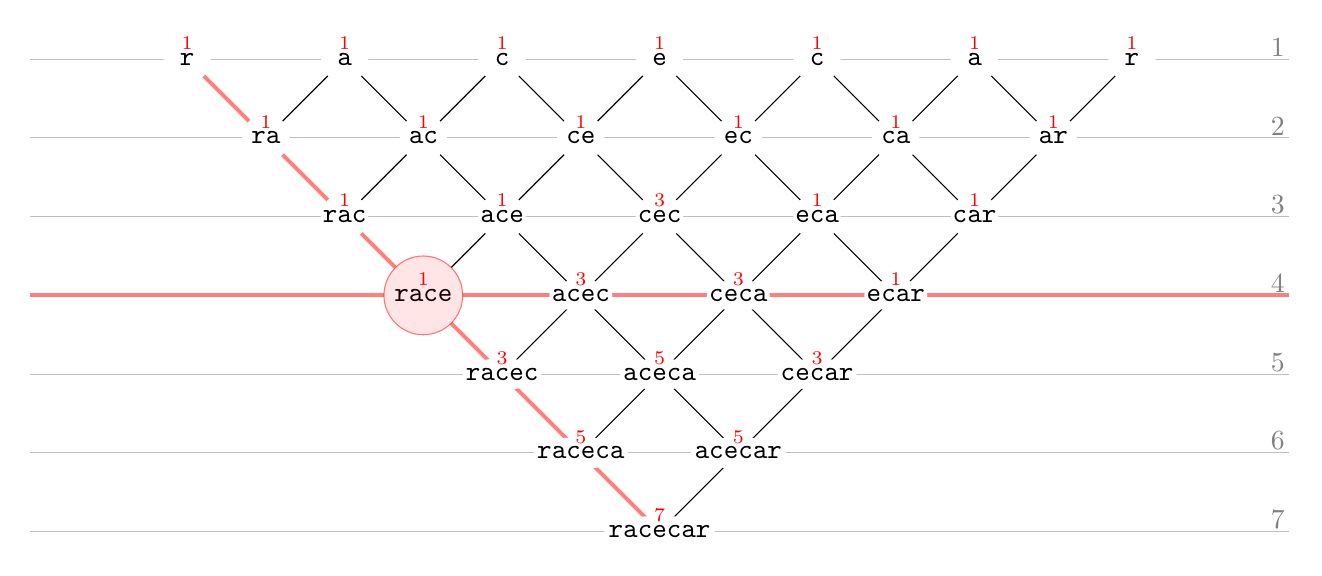
\begin{tikzpicture}
			
			\draw[red, opacity=0.5, line width=0.5mm] (-6,0) -- (0, -6);
			\draw (0,-6) -- (6,0);
			
			\draw (-4,0) -- (1,-5);
			\draw (-2,0) -- (2,-4);
			\draw (0,0) --  (3,-3);
			\draw (2,0) -- (4,-2);
			\draw (4,0) -- (5,-1);
			
			\draw (4,0) -- (-1,-5);
			\draw (2,0) -- (-2,-4);
			\draw (0,0) -- (-3,-3);
			\draw (-2,0) -- (-4,-2);
			\draw (-4,0) -- (-5,-1);
										
			\draw[opacity=0.25] (-8, 0) -- (8,0);
			\fill[fill=white] (-6,0) circle (0.3cm)
				node {\texttt{r}}
				node[anchor=south] {\scriptsize \color{red} 1};
			\fill[fill=white] (-4,0) circle (0.3cm)
				node {\texttt{a}}		
				node[anchor=south] {\scriptsize \color{red} 1};
			\fill[fill=white] (-2,0) circle (0.3cm)
				node {\texttt{c}}
				node[anchor=south] {\scriptsize \color{red} 1};			
			\fill[fill=white] (0,0) circle (0.3cm)
				node {\texttt{e}}
				node[anchor=south] {\scriptsize \color{red} 1};
			\fill[fill=white] (2,0) circle (0.3cm)
				node {\texttt{c}}
				node[anchor=south] {\scriptsize \color{red} 1};
			\fill[fill=white] (4,0) circle (0.3cm)
				node {\texttt{a}}
				node[anchor=south] {\scriptsize \color{red} 1};
			\fill[fill=white] (6,0) circle (0.3cm)
				node {\texttt{r}}
				node[anchor=south] {\scriptsize \color{red} 1};
				
			\draw[opacity=0.25] (-8, -1) -- (8,-1);
			\fill[fill=white] (-5,-1) circle (0.3cm)
				node {\texttt{ra}}
				node[anchor=south] {\scriptsize \color{red} 1};
			\fill[fill=white] (-3,-1) circle (0.3cm)
				node {\texttt{ac}}
				node[anchor=south] {\scriptsize \color{red} 1};
			\fill[fill=white] (-1,-1) circle (0.3cm)
				node {\texttt{ce}}
				node[anchor=south] {\scriptsize \color{red} 1};
			\fill[fill=white] (1,-1) circle (0.3cm)
				node {\texttt{ec}}
				node[anchor=south] {\scriptsize \color{red} 1};
			\fill[fill=white] (3,-1) circle (0.3cm)
				node {\texttt{ca}}
				node[anchor=south] {\scriptsize \color{red} 1};
			\fill[fill=white] (5,-1) circle (0.3cm)
				node {\texttt{ar}}
				node[anchor=south] {\scriptsize \color{red} 1};
				
			\draw[opacity=0.25] (-8, -2) -- (8,-2);
			\fill[fill=white] (-4,-2) circle (0.3cm)
				node {\texttt{rac}}
				node[anchor=south] {\scriptsize \color{red} 1};
			\fill[fill=white] (-2,-2) circle (0.3cm)
				node {\texttt{ace}}
				node[anchor=south] {\scriptsize \color{red} 1};
			\fill[fill=white] (0,-2) circle (0.3cm)
				node {\texttt{cec}}
				node[anchor=south] {\scriptsize \color{red} 3};		
			\fill[fill=white] (2,-2) circle (0.3cm)
				node {\texttt{eca}}
				node[anchor=south] {\scriptsize \color{red} 1};
			\fill[fill=white] (4,-2) circle (0.3cm)
				node {\texttt{car}}
				node[anchor=south] {\scriptsize \color{red} 1};
				
			\draw[red, opacity=0.5, line width=0.5mm] (-8, -3) -- (8,-3);
			\fill[fill=white] (-3,-3) circle (0.5cm)
				node {\texttt{race}}
				node[anchor=south] {\scriptsize \color{red} 1};
			\fill[red, opacity=0.1] (-3,-3) circle (0.5cm);
			\draw[red, opacity=0.5] (-3,-3) circle (0.5cm);
			\fill[fill=white] (-1,-3) ellipse (0.4cm and 0.2cm)
				node {\texttt{acec}}
				node[anchor=south] {\scriptsize \color{red} 3};
			\fill[fill=white] (1,-3) ellipse (0.4cm and 0.2cm)
				node {\texttt{ceca}}
				node[anchor=south] {\scriptsize \color{red} 3};
			\fill[fill=white] (3,-3) ellipse (0.4cm and 0.2cm)
				node {\texttt{ecar}}
				node[anchor=south] {\scriptsize \color{red} 1};
							
			\draw[opacity=0.25] (-8, -4) -- (8,-4);
			\fill[fill=white] (-2,-4) ellipse (0.5cm and 0.2cm)
				node {\texttt{racec}}
				node[anchor=south] {\scriptsize \color{red} 3};
			\fill[fill=white] (0,-4) ellipse (0.5cm and 0.2cm)
				node {\texttt{aceca}}
				node[anchor=south] {\scriptsize \color{red} 5};
			\fill[fill=white] (2,-4) ellipse (0.5cm and 0.2cm)
				node {\texttt{cecar}}
				node[anchor=south] {\scriptsize \color{red} 3};
							
			\draw[opacity=0.25] (-8, -5) -- (8,-5);
			\fill[fill=white] (-1,-5) ellipse (0.6cm and 0.2cm)
				node {\texttt{raceca}}
				node[anchor=south] {\scriptsize \color{red} 5};
			\fill[fill=white] (1,-5) ellipse (0.6cm and 0.2cm)
				node {\texttt{aceca\color{black}r}}
				node[anchor=south] {\scriptsize \color{red} 5};
				
			\draw[opacity=0.25] (-8, -6) -- (8,-6);
			\fill[fill=white] (0,-6) ellipse (0.7cm and 0.2cm)
				node {\texttt{racecar}}
				node[anchor=south] {\scriptsize \color{red} 7};
				
			\node[gray] at (8-0.15,0.15) {1};
			\node[gray] at (8-0.15,-1+0.15) {2};
			\node[gray] at (8-0.15,-2+0.15) {3};
			\node[gray] at (8-0.15,-3+0.15) {4};
			\node[gray] at (8-0.15,-4+0.15) {5};
			\node[gray] at (8-0.15,-5+0.15) {6};
			\node[gray] at (8-0.15,-6+0.15) {7};
		\end{tikzpicture}
		\caption{Identification of the substring defined by starting index 0 and depth 4}
	\end{figure}
	Now that we also have a system of coordinates in place we are 100\% set to find the solving implementation.
	\subsection{Implementation}
	\lstinputlisting[firstline=1, lastline=26, firstnumber=1, title=Implementation of the solving strategy, linewidth=18cm, xleftmargin= -1cm]{ex3tris.py}	
	\newpage
	\noindent Because I already commented my code extensively, I feel it would be useless to further explain it. However, two remarks about the structure of my code:
	\begin{itemize}
		\item I chose to use an hash-map rather than a bi-dimensional array (matrix) because I felt it would have been a wasteful use of space, since I would use only half of the space I allocate to solve this problem. 
		\item The keys of the hash-map are formatted like so \texttt{[x y]} with a non-empty space intentionally left between \texttt{x}, which is the starting index and \texttt{y} which is the length of the subsequence. This was introduced to avoid potential key conflicts and/or unwanted overwrites, as without the space between \texttt{x} and \texttt{y}, the key \texttt{111} could map to the solution for index 1 length 11 \textbf{\underline{AND}} index 11 length 1. The space solves this problem, as \texttt{"1 11"} $\neq$ \texttt{"11 1"}
	\end{itemize}
	\subsection{Time Complexity Analysis}
	Since all our operations happen on a hash-map, we can assume all our put and get operations happen in $\mathcal{O}(c)$ (although it cannot be always 100\% guaranteed due to possible hash collisions, which are still possible, even though highly unlikely). Having $n$ be defined as the length of the given string, we'll run two for loops, one for traversing the tree horizontally and one to traverse the different tree depths, corresponding to the subsequence lengths. The horizontal span of the tree is going to shrink as the length of the subsequence increases, until we just have to process a single node: the root. \\ \\
	We can be fairly sure to say that the complexity of this algorithms is $\mathcal{O}(n^2)$.
\end{homeworkExercise}
\section*{Credits}
I worked on my own throughout the whole assignment and developed all my solution autonomously.
I had some exchange of opinions as usual with \textbf{Cristian Buratti} without never seeing or trading code among ourselves. \\ \\
\textbf{Exercise 1}: Cristian actually made me realise that the problem was actually asking for subsequences, whereas I initially developed a solution to find subsets, implying that the numbers had to be consecutive. \\ \\
\textbf{Exercise 3}: The website \textbf{GeeksForGeeks} provided truly inspiring insights on how to solve this problem\footnote{\url{https://www.geeksforgeeks.org/dynamic-programming-set-12-longest-palindromic-subsequence/}}, providing also a possible \textbf{Python} solution which I decided to overlook, focusing more on the idea of having the subproblem tree and starting from the known cases to reach its root.
\section*{Attachments}
\begin{itemize}
	\item \texttt{assignment.pdf} \textemdash\ This document, did I really have to say it?
	\item \texttt{ex1.py} \textemdash\ Python file, solution to \textbf{Exercise 1}
	\item \texttt{ex2.py} \textemdash\ Python file, solution to \textbf{Exercise 2}
	\item \texttt{ex3.py} \textemdash\ Python file, solution to \textbf{Exercise 3}
\end{itemize}
\end{document}
